% !TeX spellcheck = da_DK
\documentclass[danish,a4paper,article,12pt]{article}
\documentclass{article}
\usepackage{hyperref}
\usepackage{amsmath}
\usepackage{amssymb}
\usepackage{pgfplots}
\usepackage{float}
\usepackage{todonotes}
\usepackage{tikz}

\renewcommand{\Re}{\mathbb{R}}
\newcommand{\Li}{\mathcal{L}}
\newcommand{\Ex}{\mathbb{E}}
\renewcommand{\Pr}{\mathbb{P}}
\newcommand{\Hy}{\mathcal{H}}

\newcommand\bigO[1]{
    \ensuremath{\mathcal{O}\left(#1\right)}
    }

\newcommand{\sigmoidPlot}{
    
    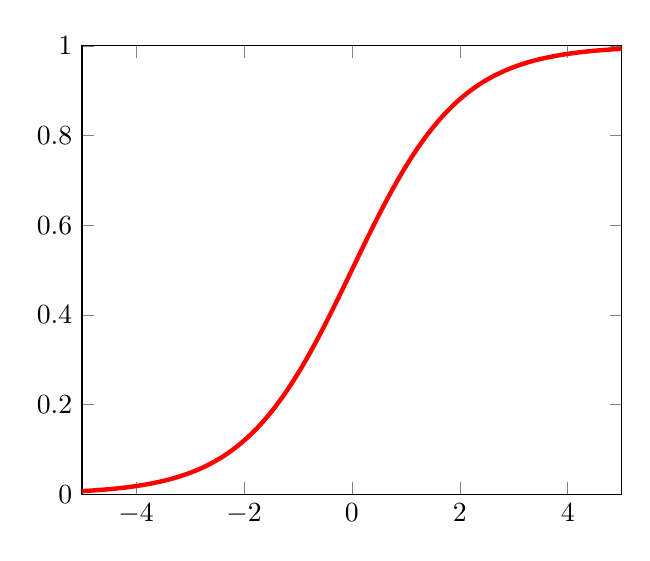
\begin{tikzpicture}
        \begin{axis}[xmin=-5, xmax=5, ymin=0, ymax=1, samples=150]
        \addplot[red, ultra thick] {1/(1+exp(-x))};
        \end{axis}
    \end{tikzpicture}
    
    }

\usetikzlibrary{positioning, calc}
\usetikzlibrary{arrows.meta}

\tikzstyle{circlebox}=[circle,thick,draw=black!75,minimum size=8mm]
\tikzstyle{inputnode}=[circlebox, draw=blue!75]
\tikzstyle{hiddennode}=[circlebox, draw=orange!75]
\tikzstyle{outputnode}=[circlebox, draw=orange!75]
\tikzstyle{simplebox}=[rectangle,thick,draw=black!75,
fill=black!20,minimum size=4mm]
\tikzstyle{textbox}=[rectangle,thick,minimum size=4mm,draw=black!0,
fill=black!0]
\tikzstyle{halfvdistance}=[yshift=-0.7cm]
\tikzstyle{abovebetween}=[xshift=-2.7mm]
\tikzstyle{edgepath} = [-Latex,->,shorten >=1pt,-stealth,semithick, rounded 
corners=5pt]

\def \nodedv {0.735cm}
\def \nodedh {0.65cm}

\tikzset{
    between/.style args={#1 and #2}{
        at = ($(#1)!0.5!(#2)$)
    }
}

\title{Cook's theorem and variants of SAT}
\author{Lukas Jørgensen, 201206057
	}
\date{\today}

\begin{document}

\maketitle

\section{Disposition}
\begin{itemize}
\item Def. af SAT og CSAT - Definér circuits
\item Red. SAT $\rightarrow$ 3SAT
\item Div. SAT-problemer - DNF, 2SAT
\item Cook's theorem - bevis
\end{itemize}

\section{Noter}
\subsection{CNF og Boolske kredsløb}

\subsubsection{CNF}
Conjective Normal Form, er en speciel afart af boolske formler. Reglerne for CNF er følgende:

\begin{enumerate}
\item De eneste tilladte funktioner er \texttt{AND, OR} og \texttt{NOT}.
\item Ingen clauses må indeholde et \texttt{AND}
\item \texttt{NOT} må kun bruges foran variable, ikke clauses.
\end{enumerate}

\subsubsection{Boolske kredsløb}
Et boolsk kredsløb er en undirected acyclic graph $G=(V,E)$, med $n$ input gates og $m$ output gates.

Der findes 4 forskellige funktionstyper for gates:
\begin{itemize}
\item[AND] tilsvarende $\wedge$.
\item[OR] tilsvarende $\vee$.
\item[NOT] tilsvarende $\neg$.
\item[COPY] der blot kopierer inputtet.
\end{itemize}

Udover disse gates, kan en gate også have en "konstant" type, der er en af de konstante symboler $\{0,1\}$ og den kan have en "variabel" type der er en af de variable symboler: $\{x_1,x_2,\dots,x_n\}$.

Der må maksimalt være én gate med et givent variabel symbol $x_j$, da disse er input-gates. Tilsvarende er der højst $m$ output-gates. Kanterne i grafen $G$ kaldes for wires. Hvis der er en wire fra gate $u$ til gate $v$ så fungerer $u$ som input til $v$.
\\
\\
Disse boolske kredsløb kan beregne en boolsk funktion $f:\{0,1\}^n\rightarrow \{0,1\}^m$, ved at evaluere kredsløbet på en given inputvektor $x\in \{0,1\}^n$. Inputvektorens værdier tildeles da til de tilsvarende inputgates.

\subsection{SAT-problemer}
\subsubsection{SAT}
\texttt{SAT} er følgende problem:
\emph{Givet en CNF formel, er der en tildeling af sandt/falsk til variablerne således at hele udtrykket evaluerer til sandt?}

\texttt{SAT} ligger i NP, da vi kan evaluere en CNF formel, med et givent input i polynomiel tid, og verificerer at resultatet er sandt eller falsk. Vi er dog nødt til at prøve alle kombinationer for rent faktisk at finde en tilfredsstillende tildeling eller at beslutte os for at der ikke er en sådan tildeling af værdier til variablerne.

\subsubsection{C-SAT}
\texttt{C-SAT} er følgende problem:
\emph{Givet et boolsk kredsløb $C$, er der en inputvektor $x\in \{0,1\}^n$ således at $C(x)=1$?}

\texttt{C-SAT} ligger i NP, da vi kan evaluere et kredsløb med en given input vektor i polynomiel tid, men vi bliver nødt til at tjekke alle mulige vektorer, for at finde ud af om der er en sådan vektor.

\subsubsection{3-SAT}
\texttt{3-SAT} er en special case af \texttt{SAT}, hvor hver clause skal indeholde præcis $3$ literals. Det er et specifikt eksempel på \texttt{k-SAT} hvor $k\geq 1$.

\subsubsection{DNF-SAT}
\texttt{DNF-SAT} er ligesom \texttt{SAT}, bortset fra at den er over DNF formler i stedet for CNF formler.

DNF formler bruger $\vee$ mellem clauses og $\wedge$ mellem literals. \texttt{DNF-SAT} ved vi ligger i $P$ (i modsætning til \texttt{SAT} som vi blot ved ligger i $NP$), da man kan tjekke hver clause for sig, og man skal blot finde én der evaluerer til sand.

\subsubsection{2-SAT}
\texttt{2-SAT} er en special case af \texttt{SAT}, hvor hver clause skal indeholde præcis $2$ literals. Det er et specifikt eksempel på \texttt{k-SAT} hvor $k\geq 1$.

\texttt{2-SAT} ved vi ligger i $P$ (i modsætning til \texttt{SAT} som vi blot ved ligger i $NP$).

For at bevise dette, konstruer en graph $G=(V,E)$ hvor der er $2n$ noder, hvor $n$ er antallet af literals, og hver node repræsenterer $x$ eller $\neg x$ for et givent literal $x$. Lav da en edge $(x_i,x_j)$ for hver clause på formen $(\neg x_i \vee x_j)$ (eller $(x_i \vee \neg x_j)$ men teknisk set er der ikke forskel). \texttt{2-SAT} formlen $\phi$ vil da være unsatisfiable hvis og kun hvis der er en sti fra $x$ til $\neg x$ og omvendt i grafen $G$.

Hvis vi antager at en sådan sti eksisterer, og $\phi$ bliver satisfied af en truth-assignment $T$. Vi ser da på en variabel $x$, hvor $T(x)=true$. Siden der er en sti fra $x$ til $\neg x$, og $T(x)=true$ mens $T(\neg x)=false$, må der være en kant $(\alpha, \beta)$ således at $T(\alpha)=true$ og $T(\beta)=false$. Men, siden $(\alpha, \beta)$ er en kant i $G$, følger det at $(\neg \alpha \vee \beta)$ er en clause i $\phi$. Denne clause er ikke satisfied af $T$, dette er en modsigelse.

Hvis vi derimod antager at der ikke eksisterer en sådan sti, så vælger vi blot en vertex der endnu ikke har fået en assignment $x$, og giver den samt alle vertices med en path fra $x$ og til disse vertices $true$, samt $false$ til de tilsvarende negeringer.

Dette step er valid, da $G$ er har en symmetri der gør at hvis der er en sti $(\alpha, \beta)$ så er der også en sti $(\neg \beta, \neg \alpha)$, så hvis der var en sti fra $x$ til både $\beta$ og $\neg \beta$, så ville der være en sti fra $x$ til $\neg x$ hvilket går imod vores antagelse.

\section{Beviser}

\subsection{Lemma 9}
\emph{Given en Turing maskine $m$ kørende i maksimalt $n \leq \rho(n)$ tid, på input af længde $n$, hvor $\rho$ er et polynomie.}

\emph{Så gælder der, at vi har et kredsløb $C_n$ med størrelsen maksimalt $O(\rho(n)^2)$, således at der gælder for alle $x\in \{0,1\}^n : C_n(x)=1$ hvis og kun hvis $M$ accepterer $x$. Derudover er funktionen der mapper $1^n$ til en beskrivelse af $C_n$ polynomielt tidsberegnelig. }

\todo[inline]{Do this shit}

\subsection{Cook's theorem}
Vi vil gerne kunne vise at diverse problemer er \texttt{NP-Complete}. Men hvis vi skal kunne gøre dette vha. reduktioner, skal vi først have et \texttt{NP-Complete} problem som vi kan reducere fra.

Stephen Cook vist i 1972 at \texttt{SAT} var \texttt{NP-Hard}, dette åbnede op for at man kunne begynde at reducere fra SAT til diverse problemer for at vise at disse nye problemer er \texttt{NP-Hard}. Oprindeligt viste Cook dette, ved at vise at alle problemer i $NP$ reducerer til \texttt{SAT}. Dette er noget omstændigt, i stedet kan man vise at \texttt{C-SAT} er \texttt{NP-Hard} og så reducere dette til \texttt{SAT}.

\subsubsection{Theorem 11 $\mathtt{C-SAT} \in NPC$}
Vi ved allerede at \texttt{C-SAT} er i $NP$. Derfor skal vi blot bevise $\mathtt{C-SAT} \in \mathtt{NP-hard}$, altså at alle sprog i $NP$ reducerer til det.

Så lad $L$ være et sprog i $NP$, nu skal vi vise at der er en reduktion $r$ således at:
\begin{equation}
\forall x : x \in L \Leftrightarrow r(x) \in \mathtt{C-SAT}
\end{equation}

Da $L\in NP$, så er der, per definition, et sprog $L'\in P$ og et polynomie $\rho$ således at:
\begin{equation}
\forall x : x \in L \Leftrightarrow \{\exists y \in \{0,1\}^* : |y| \leq \rho(x) \wedge \langle x,y \rangle \in L' \}
\end{equation}

Vores reduktion skal afbilde instanser af $L$ over i instanser af \texttt{C-SAT}, således at for et givent input $x$ så er værdien af $r(x)$ en beskrivelse af et kredsløb $C$.
Dette kredsløb, vil så indeholde $\rho(|x|)$ delkredsløb kombineret vha. $\rho(|x|)-1$ \texttt{OR-gates} således:
\begin{equation}
C \equiv D_0 \vee D_1 \vee \cdot \vee D_{\rho(|x|)}
\end{equation}
Hvert delkredsløb, bør tage $i$ Boolske inputs og evaluere dem til $1$ på inputtet $y\in \{0,1\}^i$ hvis og kun hvis $\langle x,y \rangle \in L'$ - altså kun hvis $y$ er en løsning for den givne instans. Hvis vi kan opnå at dette gælder, så er det tydeligt at $x \in L \Leftrightarrow C \in C-SAT$ som ønsket.

Delkredsløbet $D_i$ defineres således:
Lad $M$ være en Turing maskine der beslutter $L'$ i polynomiel tid. Fra Lemma 9 ved vi at, givet en fast inputlængde $n$, er der en effektiv algoritme der giver et kredsløb $C_n$ sådan at der for all $z,y$ med $|\langle z,y \rangle|=n$ har vi at $C_n( \langle z,y \rangle ) = 1$ hvis og kun hvis at $M$ acceptere $\langle z,y \rangle$.

Lad så i dette tilfælde, $n=|\langle z,y \rangle| = 2(|x|+i)+2$ for $0 \leq i \leq \rho(|x|)$.
Vores pairing funktion har formen: 
\begin{equation}
x_10x_20x_3\cdots x_{n-1}0x_n11y_10y_20y_3\cdots
\end{equation}
Derfor skal vi til slut modificere kredsløbet, således at vi kan hardcode inputtet ind i vores input gates. Således at $X_1,X_3,X_5,\dots,X_{2|x|-1}$ netop er værdierne i inputtet.\todo{måske?}. Vi ændrer da følgende gates:
\begin{description}
\item[Gate $X_{2i-1}$] erstattes med en konstant gate for bitten $x_i$.
\item[Gate $X_{2|z|+1}$] erstattes med en konstant "1" gate
\item[Gate $X_{2|z|+2}$] erstattes med en konstant "1" gate
\item[Resten] erstattes med en konstant "0" gate
\end{description}

Nu har vi at inputgatesne er hardcoded i forhold til inputtet og vores kredsløb $D_i$ er derfor nu korrekt.

Reduktionen $r$ skal således konstruere en række underkredsløb $D_0,D_1,\dots,D_{\rho(|x||)}$, kombinere dem vha. OR-gates og outputte en repræsentation af det resulterede kredsløb $C$.

Derved har vi nu en reduktion $r$ og kan derfor reducere et arbitrært sprog $L\in NP$ til \texttt{C-SAT}. så \texttt{C-SAT} er \texttt{NP-Hard}, og da vi ved at \texttt{C-SAT} desuden er i $NP$, så kan vi konkludere at $\mathtt{C-SAT} \in \mathtt{NPC}$.

\end{document}